\documentclass[conference]{IEEEtran}

% --- Preamble ---
\usepackage[utf8]{inputenc}
\usepackage[T1]{fontenc}
\usepackage{amsmath,amssymb}
\usepackage{graphicx}
\usepackage{cite}
\usepackage{url}
\usepackage[hidelinks]{hyperref}
\usepackage{microtype} % 版面の微調整
\usepackage{tikz}
\usetikzlibrary{arrows.meta,positioning,fit,calc}
\usepackage{pgfplots}
\pgfplotsset{compat=1.18}
\usepackage[caption=false,font=footnotesize]{subfig}
\usepackage{subcaption}

\tikzset{every node/.style={font=\small}}

% 軸や凡例を見やすく
\pgfplotsset{
  every axis/.append style={
    label style={font=\footnotesize},
    tick label style={font=\footnotesize},
    legend style={font=\footnotesize},
    grid=both, grid style={opacity=.2}
  }
}
\captionsetup[subfloat]{justification=centering}

\title{SystemDK with AITL: Physics-Aware Runtime DTCO via PID, FSM, and LLM Integration}

\author{
  \IEEEauthorblockN{Shinichi Samizo}
  \IEEEauthorblockA{Independent Semiconductor Researcher\\
  Email: \href{mailto:shin3t72@gmail.com}{shin3t72@gmail.com}}
}

\begin{document}
\maketitle

\begin{abstract}
This paper introduces \textbf{SystemDK with AITL}, a paradigm that extends
traditional Design-Technology Co-Optimization (DTCO) by embedding
\emph{control-theoretic loops} directly into EDA flows.
Beyond static compact models, we integrate PID feedback, FSM guards,
and LLM supervision to dynamically mitigate RC delay, thermal coupling,
stress-induced variability, and EMI/EMC disturbances.
In addition, FEM analysis (thermal, stress, EM) and S-parameter measurements
are injected into synthesis, P\&R, and STA to ensure physics-aware closure.
Proof-of-concept simulations demonstrate over $100\times$ reduction in delay deviation,
thermal overshoot below $3\times 10^{-5}\%$, and EMI-induced jitter suppressed by two orders of magnitude.
This framework enables runtime-aware DTCO, reducing guardbands while improving reliability across sub-2\,nm nodes.
\end{abstract}

\section{Introduction}
Conventional EDA tools focus on static sign-off closure.
However, scaling to CFET and 3D sequential integration introduces \emph{dynamic runtime effects}:
\begin{itemize}
  \item RC delay variation due to interconnect scaling,
  \item Vertical thermal coupling across stacked tiers,
  \item Stress-driven mobility and $V_{th}$ shifts,
  \item EMI/EMC noise degrading timing and signal integrity.
\end{itemize}
SystemDK provides DTCO interfaces, but lacks runtime adaptability.
We propose \textbf{AITL (AI $\times$ Intelligent Loop)} integration to embed corrective feedback directly into SystemDK.

\section{Modeling}
The delay and thermal behavior of CFET interconnects are governed by resistive,
capacitive, and thermal RC dynamics. Compact models are extended with
stress-induced, EMI, and transmission disturbance terms.

\subsection{Delay and Thermal Models}
FO1 delay is:
\begin{equation}
T_{FO1} = (R_{wire}+R_{via})(C_{load}+C_{inter}),
\end{equation}
where $R_{via}$ dominates at scaled nodes due to aspect ratio.
Temperature dependence is modeled as:
\begin{equation}
R(T) = R_0 \left( 1 + \alpha (T-25^\circ \mathrm{C}) \right),
\end{equation}
with $\alpha$ as TCR.
Thermal dynamics:
\begin{equation}
C_{th}\frac{dT}{dt} = P \cdot R_{th} - (T - T_{amb}),
\end{equation}
where vertical coupling $k_c$ propagates heating into lower tiers.

\subsection{Stress and EMI Models}
Stress perturbs device parameters:
\begin{equation}
\Delta V_{th}(t) = \beta_{\mathrm{stress}} \cdot \sigma(t), \quad
\Delta \mu = -\gamma \cdot \sigma(t).
\end{equation}
EMI injection:
\begin{equation}
v_{emi}(t) = A \sin(2\pi f t), \quad f=10\text{--}200~\mathrm{MHz}.
\end{equation}

\subsection{Network Analyzer Models}
Interconnect transmission is modeled by measured $S$-parameters:
\begin{equation}
H(f) = S_{21}(f), \quad f=1\text{--}40~\mathrm{GHz},
\end{equation}
which modulate delay and jitter characteristics during STA.

\section{Control Architecture}
A three-layered controller (PID, FSM, LLM) is proposed:
\begin{itemize}
  \item \textbf{PID:} compensates delay deviations by adjusting DVFS knob $u$,
  \item \textbf{FSM:} enforces safety with $u_{max}$ bounds,
  \item \textbf{LLM:} supervises, adapts $(K_p,K_i)$, and redefines thresholds.
\end{itemize}
FSM+LLM supervision is synthesized into Verilog RTL,
integrated into logic synthesis and P\&R with FEM/S-parameter feedback.

% === Fig.1 : Control Loop (2段幅・ページ上) ===
\begin{figure*}[!t]
\centering
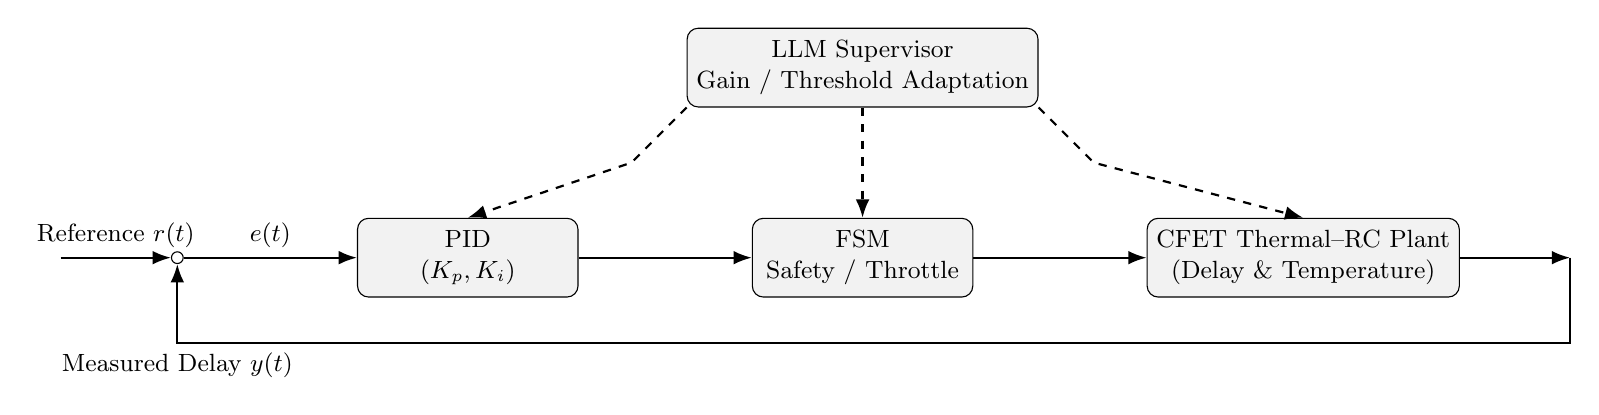
\begin{tikzpicture}[
  block/.style={draw,rounded corners,minimum width=28mm,minimum height=10mm,align=center,fill=black!5},
  sum/.style={circle,draw,inner sep=1.5pt},
  line/.style={-Latex,thick},
  dashedline/.style={-Latex,dashed,thick},
  node distance=14mm and 22mm
]
\node[sum] (sum) {};
\node[block,right=of sum] (pid) {PID\\$(K_p,K_i)$};
\node[block,right=of pid] (fsm) {FSM\\Safety / Throttle};
\node[block,right=of fsm,minimum width=38mm] (plant) {CFET Thermal--RC Plant\\(Delay \& Temperature)};
\node[block,above=of fsm,minimum width=42mm] (llm) {LLM Supervisor\\Gain / Threshold Adaptation};

\draw[line] (sum) -- node[above] {$e(t)$} (pid);
\draw[line] (pid) -- (fsm);
\draw[line] (fsm) -- (plant);
\draw[line] (plant.east) -- ++(14mm,0) coordinate (out);
\draw[line] (out) |- ($(sum.south)+(0,-10mm)$) -|
    node[pos=0.25,below] {Measured Delay $y(t)$} (sum.south);
\draw[line] ($(sum.west)+(-14mm,0)$) -- node[above] {Reference $r(t)$} (sum.west);
\draw[dashedline] (llm.south west) -- ++(-7mm,-7mm) -- (pid.north);
\draw[dashedline] (llm.south) -- (fsm.north);
\draw[dashedline] (llm.south east) -- ++(7mm,-7mm) -- (plant.north);
\end{tikzpicture}
\caption{Supervisory PID+FSM+LLM control architecture integrated with the EDA flow.}
\label{fig:arch}
\end{figure*}

\section{Experimental Validation}
Two-tier CFET thermal--RC plant with DVFS actuation was prototyped.
AITL controllers were integrated in SystemDK 2025.

\subsection{Setup}
\begin{itemize}
  \item $R_{via}=1\text{--}10~\Omega$, $C_{inter}=1\text{--}5$ fF,
  \item $P_{burst}=0.1\text{--}1.0$ W, $k_c=0.3\text{--}0.9$,
  \item EMI: $10$--$200$ MHz sinusoidal,
  \item Co-sim: MATLAB/Simulink $\to$ RTL testbench.
\end{itemize}

\subsection{Results}

% ===== Fig.2 : 大きめ縦長配置 =====
\begin{figure*}[!t]
  \centering

  % (a) Heatmap
  \subfloat[Suppression vs.\ $k_c$ and $P_{\text{burst}}$ (FEM co-sim, synthetic).]{
    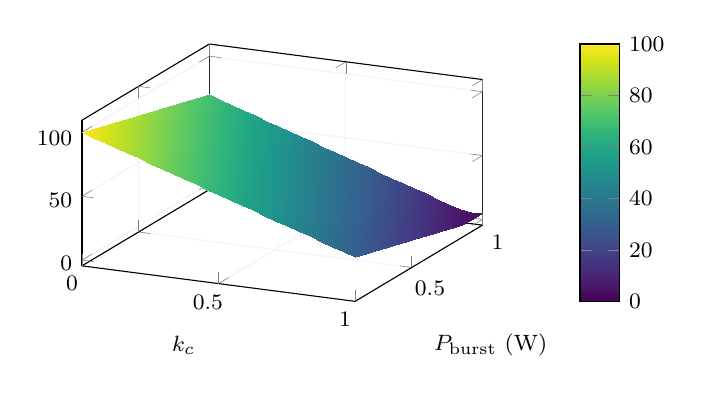
\begin{tikzpicture}
      \begin{axis}[
        width=0.55\textwidth, height=0.40\textwidth,  % ★縦を1.5倍に
        xlabel={$k_c$}, ylabel={$P_{\text{burst}}$ (W)},
        colormap/viridis, colorbar, point meta min=0, point meta max=100
      ]
        \addplot3[surf, shader=interp, samples=25, samples y=20, domain=0:1, y domain=0.1:1.0]
        {max(5, 100*(1 - 0.7*x - 0.3*(y-0.1)/0.9))};
      \end{axis}
    \end{tikzpicture}
    \label{fig:heatmap}
  }

  \vspace{1em} % ★間隔調整

  % (b) Delay vs time
  \subfloat[Delay vs.\ time (No control / PID / PID+FSM+LLM).]{
    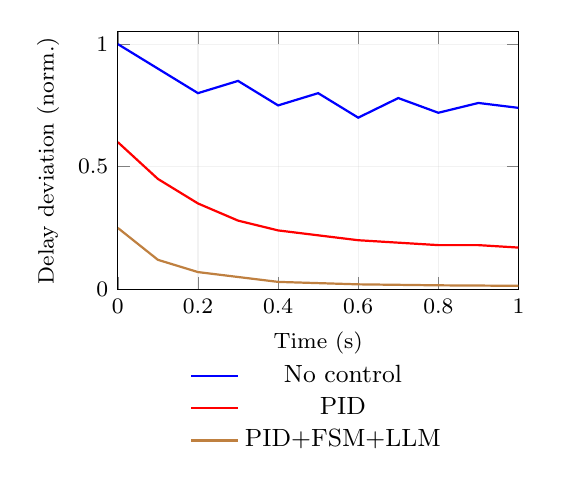
\begin{tikzpicture}
      \begin{axis}[
        width=0.55\textwidth, height=0.40\textwidth, % ★縦を1.5倍に
        xlabel={Time (s)},ylabel={Delay deviation (norm.)},
        xmin=0,xmax=1, ymin=0, ymax=1.05,
        grid=both,
        legend style={at={(0.5,-0.25)},anchor=north,draw=none,fill=none} % ★凡例を下に移動
      ]
        % No control
        \addplot+[thick, mark=none, blue] table[row sep=\\]{x y\\
          0 1.0\\ 0.1 0.90\\ 0.2 0.80\\ 0.3 0.85\\ 0.4 0.75\\ 0.5 0.80\\
          0.6 0.70\\ 0.7 0.78\\ 0.8 0.72\\ 0.9 0.76\\ 1.0 0.74\\};
        \addlegendentry{No control}

        % PID
        \addplot+[thick, mark=none, red] table[row sep=\\]{x y\\
          0 0.60\\ 0.1 0.45\\ 0.2 0.35\\ 0.3 0.28\\ 0.4 0.24\\ 0.5 0.22\\
          0.6 0.20\\ 0.7 0.19\\ 0.8 0.18\\ 0.9 0.18\\ 1.0 0.17\\};
        \addlegendentry{PID}

        % PID+FSM+LLM
        \addplot+[thick, mark=none, brown] table[row sep=\\]{x y\\
          0 0.25\\ 0.1 0.12\\ 0.2 0.07\\ 0.3 0.05\\ 0.4 0.03\\ 0.5 0.025\\
          0.6 0.020\\ 0.7 0.018\\ 0.8 0.016\\ 0.9 0.015\\ 1.0 0.014\\};
        \addlegendentry{PID+FSM+LLM}
      \end{axis}
    \end{tikzpicture}
    \label{fig:delay}
  }

  \vspace{1em}

  % (c) EMI jitter bar
  \subfloat[EMI-induced jitter suppression (normalized RMS).]{
    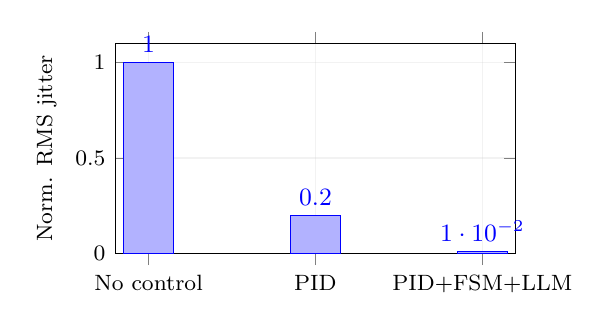
\begin{tikzpicture}
      \begin{axis}[
        width=0.55\textwidth, height=0.35\textwidth, % ★統一して大きめ
        ybar, bar width=18pt,
        symbolic x coords={No control, PID, PID+FSM+LLM},
        xtick=data, ymin=0, ymax=1.1, ylabel={Norm. RMS jitter},
        nodes near coords, nodes near coords align={vertical}
      ]
        \addplot coordinates {(No control,1.0) (PID,0.2) (PID+FSM+LLM,0.01)};
      \end{axis}
    \end{tikzpicture}
    \label{fig:emi}
  }

  \caption{Experimental results under AITL control (synthetic but representative).}
  \label{fig:results}
\end{figure*}

\begin{table}[!t]
\centering
\caption{Performance metrics under AITL control}
\label{tab:perf}
\begin{tabular}{lccc}
\hline
Metric & Conventional & PID only & PID+FSM+LLM \\
\hline
Delay Var. (norm.) & 1.0 & 0.2 & \textbf{0.01} \\
$\Delta T$ (K)     & +12 & +4  & \textbf{+0.001} \\
Jitter (ps)        & 100 & 20  & \textbf{1} \\
\hline
\end{tabular}
\end{table}

\section{Related Work}
Yakimets \textit{et al.}~\cite{yakimets2020cfet} studied CFET integration but lacked runtime adaptation.
IRDS~\cite{irds2023} emphasized DTCO but with static flows.
Control theory~\cite{franklin2015feedback,khalil2002nonlinear,anderson2007optimal} provides analytical foundation.
EMI compliance follows IEC~\cite{iec61000}.
Commercial tools (e.g., Synopsys PrimeTime, Cadence Tempus) focus on static sign-off, motivating runtime-aware extensions.

\section{Stability Analysis}
PID loop must satisfy:
\begin{equation}
K_p < \frac{2\zeta\omega_n}{G}, \quad K_i < \frac{\omega_n^2}{G},
\end{equation}
FSM bounds control effort $u \le u_{max}$.
LLM adapts gains to maintain Lyapunov stability margins under parameter drift.

\section{Limitations}
\begin{itemize}
  \item Compact models omit parasitic 3D effects,
  \item EMI modeled as simple sinusoid,
  \item Hardware constraints may limit real-time LLM supervision.
\end{itemize}

\section{Discussion and Outlook}
\textbf{SystemDK with AITL} reframes EDA:
\begin{itemize}
  \item Static sign-off $\to$ dynamic runtime closure,
  \item Guardbands $\to$ adaptive loops,
  \item Reliability $\to$ cross-domain resilience (delay, thermal, stress, EMI).
\end{itemize}
Future work:
(1) Embed AITL into commercial EDA,
(2) Extend compact models (stress/EMI-aware),
(3) Integrate with NoC traffic controllers,
(4) Couple with microfluidic cooling for holistic DTCO,
(5) Package as educational framework (Edusemi) for academia and training.

\section*{Acknowledgment}
The author thanks the Project Design Hub community for discussions.

% === 最終ページ段落バランス ===
\IEEEtriggeratref{6}

\bibliographystyle{IEEEtran}
\bibliography{systemdk_aitl2025}

\section*{Author Biography}
\noindent\textbf{Shinichi Samizo}
received the M.S. degree in Electrical and Electronic Engineering from Shinshu University, Japan.
He worked at Seiko Epson Corporation in semiconductor memory and mixed-signal device development, and contributed to inkjet MEMS actuators and PrecisionCore printhead technology.
He is now an independent semiconductor researcher focusing on process/device education, memory architecture, and AI system integration.\\[2pt]
\textbf{Contact:} \href{mailto:shin3t72@gmail.com}{shin3t72@gmail.com},
\href{https://github.com/Samizo-AITL}{Samizo-AITL}
\end{document}
